% Options for packages loaded elsewhere
\PassOptionsToPackage{unicode}{hyperref}
\PassOptionsToPackage{hyphens}{url}
\PassOptionsToPackage{dvipsnames,svgnames,x11names}{xcolor}
%
\documentclass[
  letterpaper,
  DIV=11,
  numbers=noendperiod]{scrartcl}

\usepackage{amsmath,amssymb}
\usepackage{lmodern}
\usepackage{iftex}
\ifPDFTeX
  \usepackage[T1]{fontenc}
  \usepackage[utf8]{inputenc}
  \usepackage{textcomp} % provide euro and other symbols
\else % if luatex or xetex
  \usepackage{unicode-math}
  \defaultfontfeatures{Scale=MatchLowercase}
  \defaultfontfeatures[\rmfamily]{Ligatures=TeX,Scale=1}
\fi
% Use upquote if available, for straight quotes in verbatim environments
\IfFileExists{upquote.sty}{\usepackage{upquote}}{}
\IfFileExists{microtype.sty}{% use microtype if available
  \usepackage[]{microtype}
  \UseMicrotypeSet[protrusion]{basicmath} % disable protrusion for tt fonts
}{}
\makeatletter
\@ifundefined{KOMAClassName}{% if non-KOMA class
  \IfFileExists{parskip.sty}{%
    \usepackage{parskip}
  }{% else
    \setlength{\parindent}{0pt}
    \setlength{\parskip}{6pt plus 2pt minus 1pt}}
}{% if KOMA class
  \KOMAoptions{parskip=half}}
\makeatother
\usepackage{xcolor}
\usepackage[left=1in,right=1in,top=1in]{geometry}
\setlength{\emergencystretch}{3em} % prevent overfull lines
\setcounter{secnumdepth}{-\maxdimen} % remove section numbering
% Make \paragraph and \subparagraph free-standing
\ifx\paragraph\undefined\else
  \let\oldparagraph\paragraph
  \renewcommand{\paragraph}[1]{\oldparagraph{#1}\mbox{}}
\fi
\ifx\subparagraph\undefined\else
  \let\oldsubparagraph\subparagraph
  \renewcommand{\subparagraph}[1]{\oldsubparagraph{#1}\mbox{}}
\fi

\usepackage{color}
\usepackage{fancyvrb}
\newcommand{\VerbBar}{|}
\newcommand{\VERB}{\Verb[commandchars=\\\{\}]}
\DefineVerbatimEnvironment{Highlighting}{Verbatim}{commandchars=\\\{\}}
% Add ',fontsize=\small' for more characters per line
\usepackage{framed}
\definecolor{shadecolor}{RGB}{241,243,245}
\newenvironment{Shaded}{\begin{snugshade}}{\end{snugshade}}
\newcommand{\AlertTok}[1]{\textcolor[rgb]{0.68,0.00,0.00}{#1}}
\newcommand{\AnnotationTok}[1]{\textcolor[rgb]{0.37,0.37,0.37}{#1}}
\newcommand{\AttributeTok}[1]{\textcolor[rgb]{0.40,0.45,0.13}{#1}}
\newcommand{\BaseNTok}[1]{\textcolor[rgb]{0.68,0.00,0.00}{#1}}
\newcommand{\BuiltInTok}[1]{\textcolor[rgb]{0.00,0.23,0.31}{#1}}
\newcommand{\CharTok}[1]{\textcolor[rgb]{0.13,0.47,0.30}{#1}}
\newcommand{\CommentTok}[1]{\textcolor[rgb]{0.37,0.37,0.37}{#1}}
\newcommand{\CommentVarTok}[1]{\textcolor[rgb]{0.37,0.37,0.37}{\textit{#1}}}
\newcommand{\ConstantTok}[1]{\textcolor[rgb]{0.56,0.35,0.01}{#1}}
\newcommand{\ControlFlowTok}[1]{\textcolor[rgb]{0.00,0.23,0.31}{#1}}
\newcommand{\DataTypeTok}[1]{\textcolor[rgb]{0.68,0.00,0.00}{#1}}
\newcommand{\DecValTok}[1]{\textcolor[rgb]{0.68,0.00,0.00}{#1}}
\newcommand{\DocumentationTok}[1]{\textcolor[rgb]{0.37,0.37,0.37}{\textit{#1}}}
\newcommand{\ErrorTok}[1]{\textcolor[rgb]{0.68,0.00,0.00}{#1}}
\newcommand{\ExtensionTok}[1]{\textcolor[rgb]{0.00,0.23,0.31}{#1}}
\newcommand{\FloatTok}[1]{\textcolor[rgb]{0.68,0.00,0.00}{#1}}
\newcommand{\FunctionTok}[1]{\textcolor[rgb]{0.28,0.35,0.67}{#1}}
\newcommand{\ImportTok}[1]{\textcolor[rgb]{0.00,0.46,0.62}{#1}}
\newcommand{\InformationTok}[1]{\textcolor[rgb]{0.37,0.37,0.37}{#1}}
\newcommand{\KeywordTok}[1]{\textcolor[rgb]{0.00,0.23,0.31}{#1}}
\newcommand{\NormalTok}[1]{\textcolor[rgb]{0.00,0.23,0.31}{#1}}
\newcommand{\OperatorTok}[1]{\textcolor[rgb]{0.37,0.37,0.37}{#1}}
\newcommand{\OtherTok}[1]{\textcolor[rgb]{0.00,0.23,0.31}{#1}}
\newcommand{\PreprocessorTok}[1]{\textcolor[rgb]{0.68,0.00,0.00}{#1}}
\newcommand{\RegionMarkerTok}[1]{\textcolor[rgb]{0.00,0.23,0.31}{#1}}
\newcommand{\SpecialCharTok}[1]{\textcolor[rgb]{0.37,0.37,0.37}{#1}}
\newcommand{\SpecialStringTok}[1]{\textcolor[rgb]{0.13,0.47,0.30}{#1}}
\newcommand{\StringTok}[1]{\textcolor[rgb]{0.13,0.47,0.30}{#1}}
\newcommand{\VariableTok}[1]{\textcolor[rgb]{0.07,0.07,0.07}{#1}}
\newcommand{\VerbatimStringTok}[1]{\textcolor[rgb]{0.13,0.47,0.30}{#1}}
\newcommand{\WarningTok}[1]{\textcolor[rgb]{0.37,0.37,0.37}{\textit{#1}}}

\providecommand{\tightlist}{%
  \setlength{\itemsep}{0pt}\setlength{\parskip}{0pt}}\usepackage{longtable,booktabs,array}
\usepackage{calc} % for calculating minipage widths
% Correct order of tables after \paragraph or \subparagraph
\usepackage{etoolbox}
\makeatletter
\patchcmd\longtable{\par}{\if@noskipsec\mbox{}\fi\par}{}{}
\makeatother
% Allow footnotes in longtable head/foot
\IfFileExists{footnotehyper.sty}{\usepackage{footnotehyper}}{\usepackage{footnote}}
\makesavenoteenv{longtable}
\usepackage{graphicx}
\makeatletter
\def\maxwidth{\ifdim\Gin@nat@width>\linewidth\linewidth\else\Gin@nat@width\fi}
\def\maxheight{\ifdim\Gin@nat@height>\textheight\textheight\else\Gin@nat@height\fi}
\makeatother
% Scale images if necessary, so that they will not overflow the page
% margins by default, and it is still possible to overwrite the defaults
% using explicit options in \includegraphics[width, height, ...]{}
\setkeys{Gin}{width=\maxwidth,height=\maxheight,keepaspectratio}
% Set default figure placement to htbp
\makeatletter
\def\fps@figure{htbp}
\makeatother

\setkomafont{title}{\small} \setkomafont{date}{\small}
\KOMAoption{captions}{tableheading}
\makeatletter
\makeatother
\makeatletter
\makeatother
\makeatletter
\@ifpackageloaded{caption}{}{\usepackage{caption}}
\AtBeginDocument{%
\ifdefined\contentsname
  \renewcommand*\contentsname{Table of contents}
\else
  \newcommand\contentsname{Table of contents}
\fi
\ifdefined\listfigurename
  \renewcommand*\listfigurename{List of Figures}
\else
  \newcommand\listfigurename{List of Figures}
\fi
\ifdefined\listtablename
  \renewcommand*\listtablename{List of Tables}
\else
  \newcommand\listtablename{List of Tables}
\fi
\ifdefined\figurename
  \renewcommand*\figurename{Figure}
\else
  \newcommand\figurename{Figure}
\fi
\ifdefined\tablename
  \renewcommand*\tablename{Table}
\else
  \newcommand\tablename{Table}
\fi
}
\@ifpackageloaded{float}{}{\usepackage{float}}
\floatstyle{ruled}
\@ifundefined{c@chapter}{\newfloat{codelisting}{h}{lop}}{\newfloat{codelisting}{h}{lop}[chapter]}
\floatname{codelisting}{Listing}
\newcommand*\listoflistings{\listof{codelisting}{List of Listings}}
\makeatother
\makeatletter
\@ifpackageloaded{caption}{}{\usepackage{caption}}
\@ifpackageloaded{subcaption}{}{\usepackage{subcaption}}
\makeatother
\makeatletter
\@ifpackageloaded{tcolorbox}{}{\usepackage[many]{tcolorbox}}
\makeatother
\makeatletter
\@ifundefined{shadecolor}{\definecolor{shadecolor}{rgb}{.97, .97, .97}}
\makeatother
\makeatletter
\makeatother
\ifLuaTeX
  \usepackage{selnolig}  % disable illegal ligatures
\fi
\IfFileExists{bookmark.sty}{\usepackage{bookmark}}{\usepackage{hyperref}}
\IfFileExists{xurl.sty}{\usepackage{xurl}}{} % add URL line breaks if available
\urlstyle{same} % disable monospaced font for URLs
\hypersetup{
  pdftitle={Normal distribution},
  colorlinks=true,
  linkcolor={blue},
  filecolor={Maroon},
  citecolor={Blue},
  urlcolor={Blue},
  pdfcreator={LaTeX via pandoc}}

\title{Normal distribution}
\author{}
\date{}

\begin{document}
\maketitle
\ifdefined\Shaded\renewenvironment{Shaded}{\begin{tcolorbox}[enhanced, breakable, boxrule=0pt, borderline west={3pt}{0pt}{shadecolor}, sharp corners, frame hidden, interior hidden]}{\end{tcolorbox}}\fi

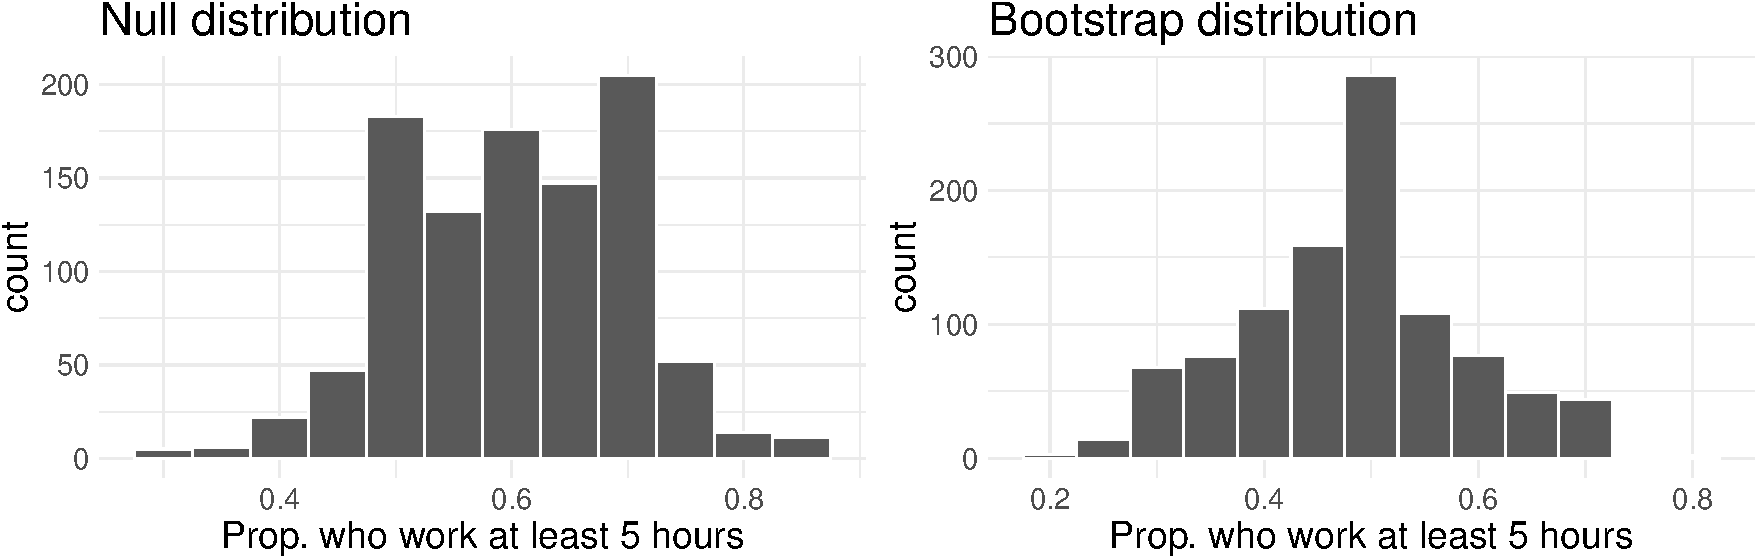
\includegraphics{worksheet-16-normal_files/figure-pdf/unnamed-chunk-3-1.pdf}

\hypertarget{rules}{%
\subsection{68-95-99.7 rules}\label{rules}}

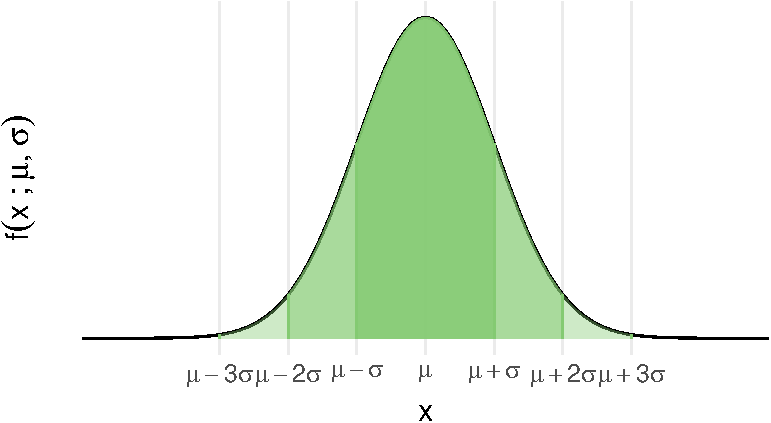
\includegraphics{worksheet-16-normal_files/figure-pdf/unnamed-chunk-4-1.pdf}

\hypertarget{finding-areas}{%
\subsection{Finding areas}\label{finding-areas}}

Suppose \(X \sim N(0,1)\)

\begin{figure}

\begin{minipage}[t]{0.33\linewidth}

{\centering 

Area less than -2 and greater than 2.

}

\end{minipage}%
%
\begin{minipage}[t]{0.33\linewidth}

{\centering 

Area between 0 and 1.

}

\end{minipage}%
%
\begin{minipage}[t]{0.33\linewidth}

{\centering 

Area to the right of 1.

}

\end{minipage}%
\newline
\begin{minipage}[t]{0.33\linewidth}

{\centering 

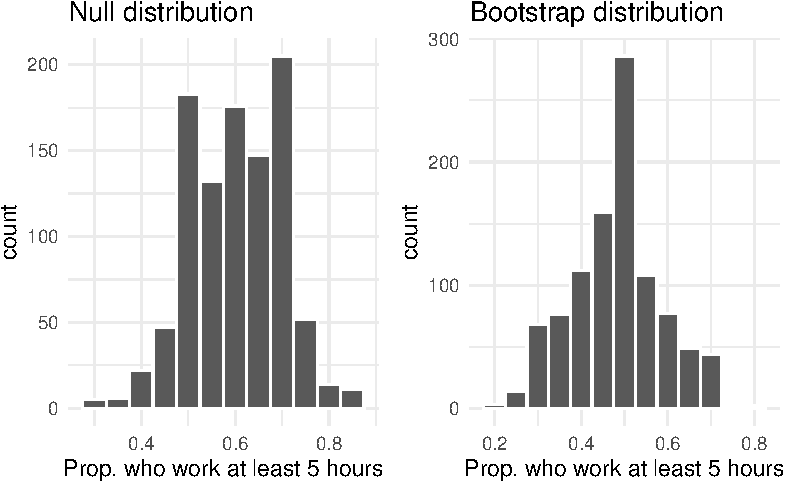
\includegraphics{worksheet-16-normal_files/figure-pdf/unnamed-chunk-5-1.pdf}

}

\end{minipage}%
%
\begin{minipage}[t]{0.33\linewidth}

{\centering 

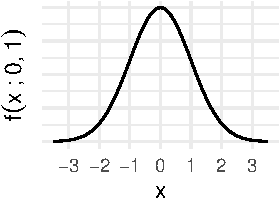
\includegraphics{worksheet-16-normal_files/figure-pdf/unnamed-chunk-6-1.pdf}

}

\end{minipage}%
%
\begin{minipage}[t]{0.33\linewidth}

{\centering 

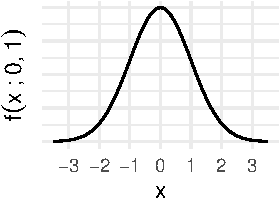
\includegraphics{worksheet-16-normal_files/figure-pdf/unnamed-chunk-7-1.pdf}

}

\end{minipage}%
\newline
\begin{minipage}[t]{0.33\linewidth}

{\centering 

\(\quad\)

}

\end{minipage}%
%
\begin{minipage}[t]{0.33\linewidth}

{\centering 

\(\quad\)

}

\end{minipage}%
%
\begin{minipage}[t]{0.33\linewidth}

{\centering 

\(\quad\)

}

\end{minipage}%
\newline
\begin{minipage}[t]{0.33\linewidth}

{\centering 

\(\text{P}(\qquad\qquad\qquad) \approx\)

}

\end{minipage}%
%
\begin{minipage}[t]{0.33\linewidth}

{\centering 

\(\quad\)

}

\end{minipage}%
%
\begin{minipage}[t]{0.33\linewidth}

{\centering 

\(\quad\)

}

\end{minipage}%

\end{figure}

\vspace{4cm}

\hypertarget{z-score-problem}{%
\subsection{Z-score problem}\label{z-score-problem}}

The distribution of SAT and ACT scores are both nearly Normal. The SAT
has a mean of 1100 and standard deviation of 200, while the ACT has a
mean of 21 and standard deviation of 6. Suppose Ann scored 1300 on her
SAT and Tom scored 24 on his ACT. Who performed better?

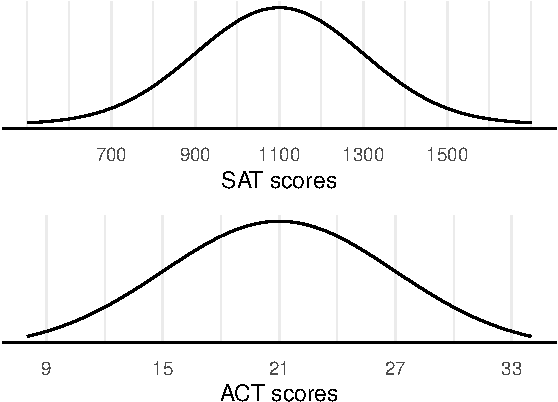
\includegraphics{worksheet-16-normal_files/figure-pdf/unnamed-chunk-8-1.pdf}

\clearpage

\hypertarget{percentiles}{%
\subsection{Percentiles}\label{percentiles}}

\begin{figure}

\begin{minipage}[t]{0.50\linewidth}

{\centering 

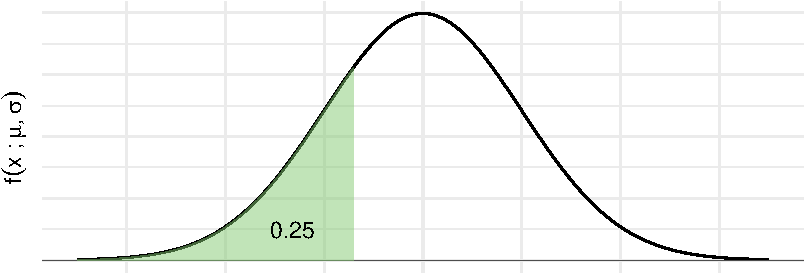
\includegraphics{worksheet-16-normal_files/figure-pdf/unnamed-chunk-9-1.pdf}

}

\end{minipage}%
%
\begin{minipage}[t]{0.50\linewidth}

{\centering 

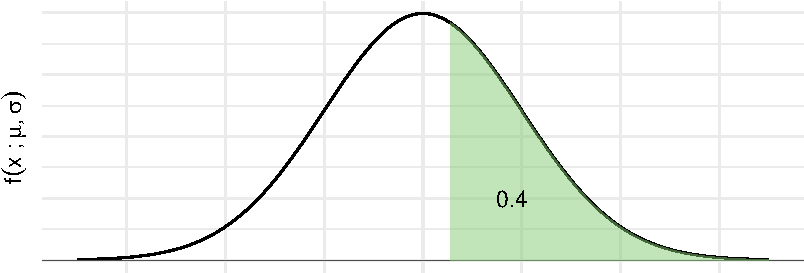
\includegraphics{worksheet-16-normal_files/figure-pdf/unnamed-chunk-10-1.pdf}

}

\end{minipage}%
\newline
\begin{minipage}[t]{0.50\linewidth}

{\centering 

\begin{Shaded}
\begin{Highlighting}[]
\FunctionTok{qnorm}\NormalTok{(}\FloatTok{0.25}\NormalTok{, }\AttributeTok{mean =}\NormalTok{ mu, }\AttributeTok{sd =}\NormalTok{ sigma)}
\end{Highlighting}
\end{Shaded}

}

\end{minipage}%
%
\begin{minipage}[t]{0.50\linewidth}

{\centering 

}

\end{minipage}%

\end{figure}

\hypertarget{percentile-problems}{%
\subsection{Percentile problems}\label{percentile-problems}}

Suppose SAT scores are Normally distributed with mean 1100 and standard
deviation 200.

\begin{enumerate}
\def\labelenumi{\arabic{enumi}.}
\tightlist
\item
  Edward earned a 1030 on his SAT. We will find his percentile using
  code in two ways.

  \begin{enumerate}
  \def\labelenumii{\alph{enumii}.}
  \tightlist
  \item
    First, draw a picture representing what we want to find. Then write
    code to find the percentile.
  \item
    Find Edward's z-score. Write another line of code to find the
    percentile.
  \end{enumerate}
\item
  What is the 97.5th percentile for SAT scores?

  \begin{enumerate}
  \def\labelenumii{\alph{enumii}.}
  \tightlist
  \item
    Write code to answer this question.
  \item
    Write a different line of code to answer this question that involves
    a z-score.
  \end{enumerate}
\item
  Unrelated to SAT scores: consider the standard normal \(N(0,1)\)
  distribution. The 25th percentile of this distribution is -0.67.
  Without doing any work beyond drawing a picture, what is the 75th
  percentile of the distribution?
\end{enumerate}

\clearpage

\hypertarget{some-practice-problems}{%
\subsection{Some practice problems}\label{some-practice-problems}}

\begin{enumerate}
\def\labelenumi{\arabic{enumi}.}
\item
  In a law school class, the entering students averaged 160 on the LSAT.
  The variance was 64. The histogram of LSAT scores followed the normal
  curve reasonable well.

  \begin{enumerate}
  \def\labelenumii{\alph{enumii}.}
  \item
    About what percentage of the class scores below 152?
  \item
    One student was 0.5 standard deviations above average on the LSAT.
    About what percentage of the students had lower scores than he did?
  \end{enumerate}
\item
  Weights of 10-year-old girls are known to be Normally distributed with
  mean of 70 pounds and standard deviation of 13 pounds. Find the
  probability that a 10-year-old girl weighs between 60 and 85 pounds
  two ways:

  \begin{enumerate}
  \def\labelenumii{\alph{enumii}.}
  \item
    Optional, but helpful: draw a sketch of the curve and shade in the
    region of interest.
  \item
    Write the probability of interest in \(P()\) form. Then write the
    \texttt{R} code necessary to find this probability, and actually
    execute the code to obtain the probability.
  \item
    Confirm your solution in (b) by transforming to z-scores first, then
    using code again to obtain the probability.
  \end{enumerate}
\item
  Consider the same scenario as in 2. Without using any code than what
  is provided below, find the 60th percentile for the weight of
  10-year-old girls.

\begin{Shaded}
\begin{Highlighting}[]
\FunctionTok{qnorm}\NormalTok{(}\FloatTok{0.6}\NormalTok{, }\AttributeTok{mean =} \DecValTok{0}\NormalTok{, }\AttributeTok{sd =} \DecValTok{1}\NormalTok{)}
\end{Highlighting}
\end{Shaded}

\begin{verbatim}
[1] 0.2533471
\end{verbatim}
\item
  \((^*)\) Suppose body temperatures are Normally distributed with mean
  \(98.6^\circ\) F and standard deviation of \(0.7^\circ\) F. Assuming
  this is true, answer the following:

  \begin{enumerate}
  \def\labelenumii{\alph{enumii}.}
  \item
    Fevers \(103^\circ\) F or higher are considered dangerous. What
    fraction of people would be expected to have such high a fever?
  \item
    According to quick Google search, a range for low-grade fever is
    between \(99.5^\circ\) F and \(100.3^\circ\) F. What is the
    probability of having a low-grade fever?
  \item
    What body temperatures would you consider as unusually low? Briefly
    explain why.
  \item
    Provide two intervals that each capture/contain 80\% of body
    temperatures.
  \end{enumerate}
\end{enumerate}



\end{document}
